\documentclass{article}

\usepackage[margin=1.0in]{geometry}
\usepackage{graphicx}
\usepackage{amsmath}
\usepackage{float}
\usepackage{enumitem}
\usepackage{gensymb}

\title{CSC 577 HW4}
\date{2/13/2019}
\author{Simon Swenson}

\begin{document}

\pagenumbering{gobble}
\maketitle
\pagenumbering{arabic}

\section{Introduction}

In this assignment, we explored the typical pixel coordinate system of images and how 
that relates to MATLAB's matrix indexing. We also generated some ground truth 
data by labeling various grid vertices on the calibration image. These ground 
truth points were then used to compare two proposed camera matrices, both 
visually and statistically (using RMSE). Finally, in the grad portion section, 
properties of simple transformation matrices, like translation matrices, were 
explored, and a series of simple transformation matrices were combined to create 
a transformation from standard coordinates to image coordinates.

\section{Clicking Coordinates and Image Location}

\begin{figure}[!ht]
	\centering
	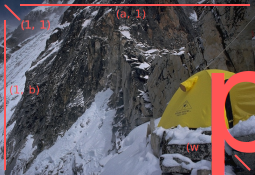
\includegraphics[width=120mm]{figs/tent_labeled.png}
	\caption{Here, we see the familiar tent image. If you are at all familiar 
        with images, the coordinate space in which they're typically represented 
        is no surprise. Thankfully, MATLAB's click coordinate system follows the 
        typical coordinate system. Lower x coordinates appear farther to the left, lower y 
        coordinates 
        appear farther to the top. It is essentially a 2-d grid arranged from top-left 
        to bottom-right. However, one caveat is that the pixel at the top-left 
        is given by coordinate (1, 1) rather than (0, 0). This is atypical for 
        image manipulation tasks. It is likely an artifact of MATLAB's base-1 
        indexing. This also means that the coordinate for the bottom-right is 
        given by (w, h), where w is the image width in pixels and h is the image 
        height in pixels.}
\end{figure}

\subsection{Click Coordinates to MATLAB Matrix Coordinates}

Recall that MATLAB uses the standard mathematical ordering for matrix indexing: 
row-major order. However, the matrix in MATLAB is stored exactly how it appears 
on screen (ignoring the channel, for now). This means that columns index x 
coordinates and rows index y coordinates. Due to the row-major indexing, this 
means that \textit{y coordinates are indexed first}. So, to refer to the clicked 
pixel $(p_x, p_y)$, one would have to index in MATLAB like so: $tent\_image(p_y, p_x, :)$. 
In other words, just flip the order of the x and y coordinate.

\begin{figure}[!ht]
	\centering
	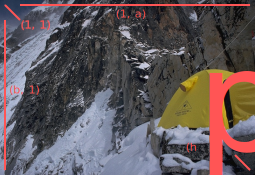
\includegraphics[width=120mm]{figs/tent_labeled_2.png}
	\caption{Here is the same tent image, this time represented with coordinates 
        in terms of MATLAB matrices. Notice that all coordinates are reversed, 
        with y coordinate first, followed by the x coordinate.}
\end{figure}

\section{Labeled Coordinate Data}

To calibrate the camera, we need a certain number of labeled points. Our 
equation has 11 unknowns, so we need at least 11 linear equations to obtain a 
good result. This will give us an exact answer, but, as our measurements are not 
perfect, it may not be a \textit{good} answer. The solution, as is often the 
case in data science, is to add more data points. Thus, we pick 15 points in the 
calibration image. The points picked can be found in an image and chart nearby.

\begin{figure}[!ht]
	\centering
	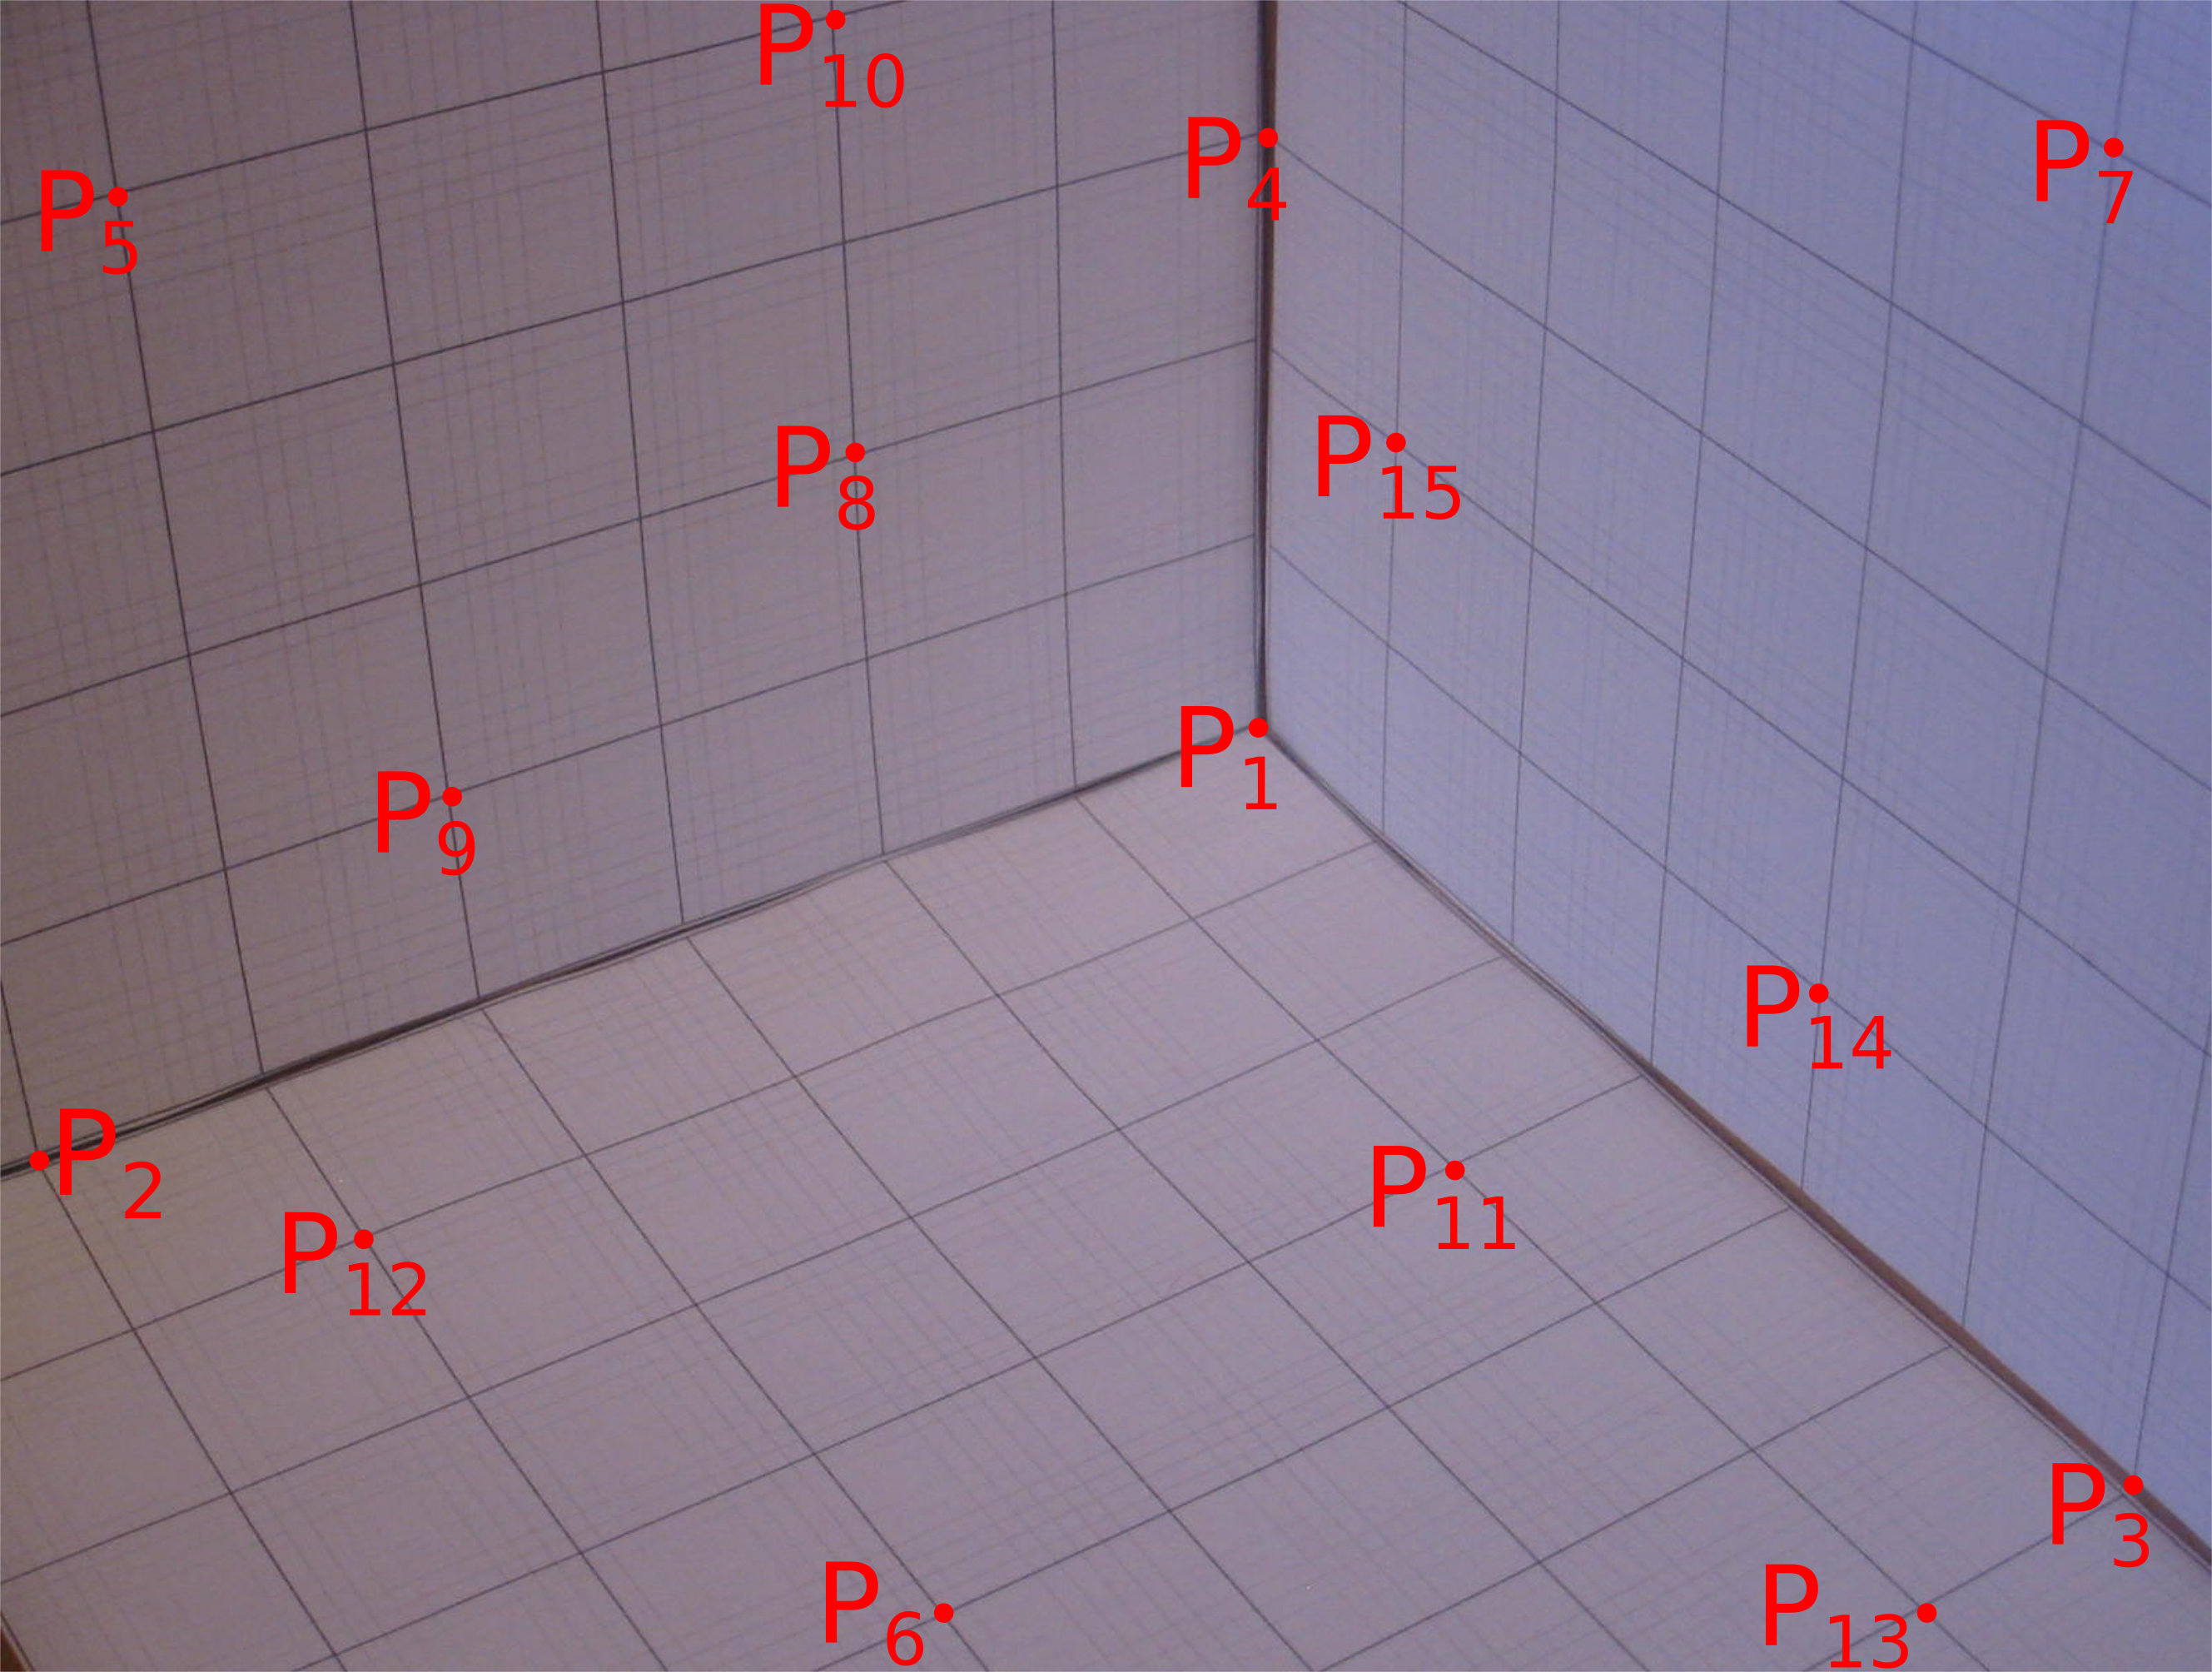
\includegraphics[width=120mm]{figs/calibration_labeled.png}
	\caption{The fifteen points chosen for calibration.}
\end{figure}

\begin{tabular}{c | c c}
    Point    & World Coordinates & Image Coordinates \\
    \hline \\
    $P_1$    & (0.0, 0.0, 0.0) & ( \enspace         521, \enspace         913) \\
    $P_2$    & (6.0, 0.0, 0.0) & ( \enspace         832, \enspace \enspace 27) \\
    $P_3$    & (0.0, 6.0, 0.0) & (                 1071,                 1541) \\
    $P_4$    & (0.0, 0.0, 3.0) & ( \enspace \enspace 98, \enspace         916) \\
    $P_5$    & (5.0, 0.0, 4.0) & ( \enspace         138, \enspace \enspace 85) \\
    $P_6$    & (4.0, 4.0, 0.0) & (                 1159, \enspace         682) \\
    $P_7$    & (0.0, 5.0, 5.0) & ( \enspace         110,                 1530) \\
    $P_8$    & (2.0, 0.0, 2.0) & ( \enspace         329, \enspace         618) \\
    $P_9$    & (4.0, 0.0, 1.0) & ( \enspace         569, \enspace         324)  \\
    $P_{10}$ & (2.0, 0.0, 4.0) & ( \enspace \enspace 12, \enspace         603)  \\
    $P_{11}$ & (1.0, 3.0, 0.0) & ( \enspace         835,                 1051)  \\
    $P_{12}$ & (5.0, 1.0, 0.0) & ( \enspace         885, \enspace         262)  \\
    $P_{13}$ & (1.0, 6.0, 0.0) & (                 1153,                 1389)  \\
    $P_{14}$ & (6.0, 4.0, 1.0) & ( \enspace         713,                 1318)  \\
    $P_{15}$ & (6.0, 1.0, 2.0) & ( \enspace         318,                 1010)
\end{tabular}

\section{Several Proposed Camera Matrices}

\subsection{Qualitative Results: A Visual Inspection}

Suppose we have labeled data and a proposed camera matrix. How can we determine 
how good that camera matrix is? One way is through visual inspection: Simply 
send world points through the matrix to get image points, and inspect those 
image points in comparison to the ground truth. Doing so with the two provided 
example matrices shows that, while neither is perfect, the first one (green 
dots) has output that is much closer to the 
ground truth than the second matrix (blue dots).

\begin{figure}[!ht]
	\centering
	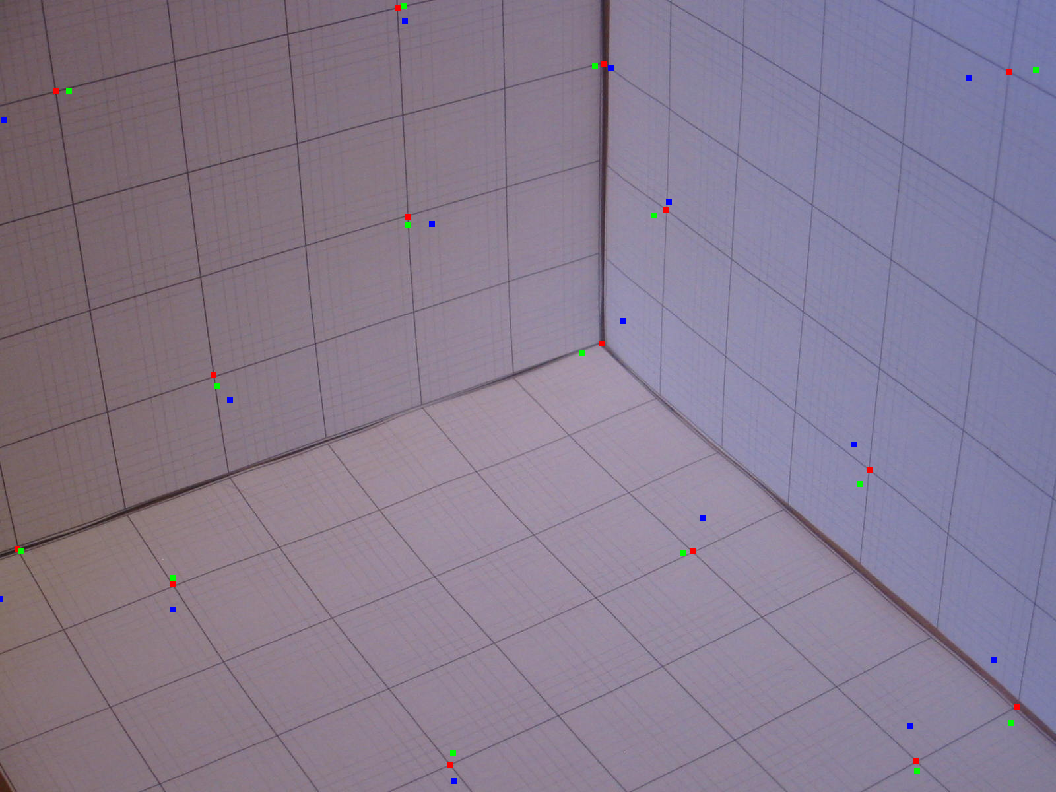
\includegraphics[width=120mm]{figs/projected_points.png}
	\caption{The original fifteen ground truth points (again, appearing red), 
        now alongside the projections of two proposed camera matrices. The green 
        dots seem to be closer in most cases, so, visually, the green matrix 
        (the first of the two) appears to be better.}
\end{figure}

\subsection{Quantitative Results: A Comparison of Errors}

In addition to the qualitative visual analysis, we can simply calculate the 
RMSE of the projections. Recall that the RMSE is given by:

$$
RMSE = \sqrt{\frac{\sum_i distance(y_i, M x_i)^2}{N}}
$$

Where $distance$ is the standard Euclidean distance metric:

$$
distance(p_1, p_2) = \sqrt{\sum_d (p_{1, d} - p_{2, d})^2}
$$

$y_i$ is the ground truth projection for point $i$, $ M $ is the camera 
matrix, and $x_i$ is the position for point $i$ in world space. Note that 
squared distance cancels the square root in the distance formula, so we just 
have:

$$
RMSE = \sqrt{\frac{\sum_i \sum_d (x_{i,d} - y_{i, d})^2}{N}}
$$

The results are as follows:

\begin{tabular}{r | r}
    Matrix 1 RMSE & 20.9578 \\
    Matrix 2 RMSE & 52.1719
\end{tabular}

Thus, as expected by our visual inspection, the first matrix (green) is 
significantly better than the second one.

\section{Results and Properties for Translation Matrices}

\subsection{Inverse}

Intuitively, a translation is undone by simply translating in the opposite 
direction. Thus, a proposal for the inverse of a matrix M, where

$$
T = \begin{bmatrix}
1 & 0 & 0 & t_x \\
0 & 1 & 0 & t_y \\
0 & 0 & 1 & t_z \\
0 & 0 & 0 & 1
\end{bmatrix}
$$

is:

$$
T' = \begin{bmatrix}
1 & 0 & 0 & -t_x \\
0 & 1 & 0 & -t_y \\
0 & 0 & 1 & -t_z \\
0 & 0 & 0 & 1
\end{bmatrix}
$$

Proof:

$$
T T' = \begin{bmatrix}
1 & 0 & 0 & t_x \\
0 & 1 & 0 & t_y \\
0 & 0 & 1 & t_z \\
0 & 0 & 0 & 1
\end{bmatrix} \begin{bmatrix}
1 & 0 & 0 & -t_x \\
0 & 1 & 0 & -t_y \\
0 & 0 & 1 & -t_z \\
0 & 0 & 0 & 1
\end{bmatrix} = \begin{bmatrix}
1 & 0 & 0 & -t_x + t_x \\
0 & 1 & 0 & -t_y + t_y \\
0 & 0 & 1 & -t_z + t_z \\
0 & 0 & 0 & 1
\end{bmatrix} = I_4
$$

\subsection{Commutativity}

Claim: Translation matrices are commutative.

Proof: The key to this proof is that addition is commutative. Let

$$
T = \begin{bmatrix}
1 & 0 & 0 & t_x \\
0 & 1 & 0 & t_y \\
0 & 0 & 1 & t_z \\
0 & 0 & 0 & 1
\end{bmatrix}
$$

and

$$
U = \begin{bmatrix}
1 & 0 & 0 & u_x \\
0 & 1 & 0 & u_y \\
0 & 0 & 1 & u_z \\
0 & 0 & 0 & 1
\end{bmatrix}
$$

By inspection, they are both translation matrices. Then

$$
T U = \begin{bmatrix}
1 & 0 & 0 & t_x \\
0 & 1 & 0 & t_y \\
0 & 0 & 1 & t_z \\
0 & 0 & 0 & 1
\end{bmatrix} \begin{bmatrix}
1 & 0 & 0 & u_x \\
0 & 1 & 0 & u_y \\
0 & 0 & 1 & u_z \\
0 & 0 & 0 & 1
\end{bmatrix} = \begin{bmatrix}
1 & 0 & 0 & u_x + t_x \\
0 & 1 & 0 & u_y + t_y \\
0 & 0 & 1 & u_z + t_z \\
0 & 0 & 0 & 1
\end{bmatrix}
$$

Using modus ponens on the immediate above result of $ T U $ with $ U T $, we 
arrive at:
$$
U T = \begin{bmatrix}
1 & 0 & 0 & t_x + u_x \\
0 & 1 & 0 & t_y + u_y \\
0 & 0 & 1 & t_z + u_z \\
0 & 0 & 0 & 1
\end{bmatrix}
$$

which equals $ T U $ by the commutativity of addition.

\subsection{Translation with Non-1 Homogeneous Coordinates}

Consider a point in homogeneous coordinates 

$$
P_h = \begin{bmatrix}
a \\
b \\
c \\
w
\end{bmatrix}
$$

Then, by the conversion function,

$$
P = \begin{bmatrix}
\frac{a}{w} \\
\frac{b}{w} \\
\frac{c}{w}
\end{bmatrix}
$$

Consider a naive translation, that is, one that does not use a matrix, on point 
$P$:

$$
P + t = \begin{bmatrix}
\frac{a}{w} \\
\frac{b}{w} \\
\frac{c}{w}
\end{bmatrix} + \begin{bmatrix}
t_x \\
t_y \\
t_z
\end{bmatrix} = \begin{bmatrix}
\frac{a}{w} + t_x \\
\frac{b}{w} + t_y\\
\frac{c}{w} + t_z
\end{bmatrix}
$$

Now, consider a translation by a matrix in homogeneous coordinates:

$$
T P_h = \begin{bmatrix}
1 & 0 & 0 & t_x \\
0 & 1 & 0 & t_y \\
0 & 0 & 1 & t_z \\
0 & 0 & 0 & 1
\end{bmatrix} \begin{bmatrix}
a \\
b \\
c \\
w
\end{bmatrix} = \begin{bmatrix}
a + w t_x \\
b + w t_y \\
c + w t_z \\
w
\end{bmatrix}
$$

Then, applying the conversion to the standard coordinate system, we have:

$$\begin{bmatrix}
a + w t_x \\
b + w t_y \\
c + w t_z \\
w
\end{bmatrix} \rightarrow \begin{bmatrix}
\frac{a + w t_x}{w} \\
\frac{b + w t_y}{w} \\
\frac{c + w t_z}{w} \\
\end{bmatrix} = \begin{bmatrix}
\frac{a}{w} + t_x \\
\frac{b}{w} + t_y \\
\frac{c}{w} + t_z \\
\end{bmatrix}
$$

This proves the equivalence.

\section{A Standard Mapping between Image Pixel Coordinates and the Standard XY Coordinate System}

In order to find a map between standard coordinates and pixel coordinates, we'll 
need to come up with 
some set of matrices which represent the primitive transformations, then we'll 
figure out the ordering needed to achieve 
the output that we want. Let's start with the transformation from standard coordinates 
to image coordinates. One matrix that we'll need is a translation matrix. Since we want 
(0, 0) to map to (400, 600), we'll define that matrix:

$$
M_t = \begin{bmatrix}
1 & 0 & 400 \\
0 & 1 & 600 \\
0 & 0 &   1
\end{bmatrix}
$$

Another matrix we'll need is the scaling matrix. Since we want one unit in 
standard coordinates to correspond to 400 pixels (in both directions), we have 
the matrix:

$$
M_s = \begin{bmatrix}
400 &   0 & 0 \\
  0 & 400 & 0 \\
  0 &   0 & 1
\end{bmatrix}
$$

Finally, we'll need to flip the vertical direction, since pixels increase going 
down, and standard coordinates decrease going down:

$$
M_f = \begin{bmatrix}
1 &  0 & 0 \\
0 & -1 & 0 \\
0 &  0 & 1
\end{bmatrix}
$$

Now, the order of these matrices are important, since matrix multiplication is 
not necessarily commutative. We want to perform the flip when the coordinate 
system is still centered, or our y coordinate ranges could end up going to the 
interval [-1200, 0] instead of [0, 1200]. so we'll perform that first. Now, if 
we perform translation before scaling, we'll move the relatively small interval 
[-1, 1] out to some obscenely large coordinate [-399, 401]. Then, when we scale, 
we will have a giant dead area between the origin and this region. Thus, 
we'll perform the scaling, then finally the translation.

$$
M = M_t M_s M_f = \begin{bmatrix}
1 & 0 & 400 \\
0 & 1 & 600 \\
0 & 0 &   1
\end{bmatrix} \begin{bmatrix}
400 &   0 & 0 \\
  0 & 400 & 0 \\
  0 &   0 & 1
\end{bmatrix} \begin{bmatrix}
1 &  0 & 0 \\
0 & -1 & 0 \\
0 &  0 & 1
\end{bmatrix} = \begin{bmatrix}
400 &    0 & 400 \\
  0 & -400 & 600 \\
  0 &    0 & 1
\end{bmatrix}
$$

Here's some sample points. We expect (-0.5, -0.5) to hit near (200, 800), 
(-0.5, 0.5) near (200, 400), (0, 1) near (400, 200).

$$
\begin{bmatrix}
400 &    0 & 400 \\
  0 & -400 & 600 \\
  0 &    0 & 1
\end{bmatrix} \begin{bmatrix}
-0.5\\
-0.5\\
1
\end{bmatrix} = \begin{bmatrix}
200\\
800\\
1
\end{bmatrix}
$$

$$
\begin{bmatrix}
400 &    0 & 400 \\
  0 & -400 & 600 \\
  0 &    0 & 1
\end{bmatrix} \begin{bmatrix}
-0.5\\
 0.5\\
1
\end{bmatrix} = \begin{bmatrix}
200\\
400\\
1
\end{bmatrix}
$$

$$
\begin{bmatrix}
400 &    0 & 400 \\
  0 & -400 & 600 \\
  0 &    0 & 1
\end{bmatrix} \begin{bmatrix}
0\\
1\\
1
\end{bmatrix} = \begin{bmatrix}
400\\
200\\
1
\end{bmatrix}
$$

We're getting the expected results, so our transformation looks good!

\section{Conclusion}

In this lesson, we saw the relationship between the traditional way of indexing 
image pixels, using (x, y) order and starting at the top-left of the image and 
MATLAB matrix indices, namely, that the x and y values needed 
to be flipped lexicographically. We spent 
some time simulating a Mechanical Turk session by generating labeled data, 
coordinates in world space (using the grid lines on the calibration image) and 
matching pixel coordinates (by MATLAB's data selection tool). We used this 
ground truth to compare two propsed camera matrices. Upon visual inspection, the 
green matrix (first matrix) was found to be better, which was backed up by our 
RMSE measurement. After that, we proved some properties of translation matrices. 
Finally, alongside one such translation matrix, we used other primitive matrices like a 
flip matrix and a scale matrix to perform a more complicated operation, 
converting from standard image coordinates to 
pixel coordinates.

\end{document}